\documentclass[12pt]{letter}\usepackage[letterpaper,margin=0.65in]{geometry}\usepackage{textcomp}\usepackage{graphicx}\usepackage[rflt]{floatflt}\pagenumbering{gobble}\begin{document}\begin{floatingfigure}{0.15\textwidth}\raisebox{0pt}[0pt][0pt]{\raisebox{-2.5cm}{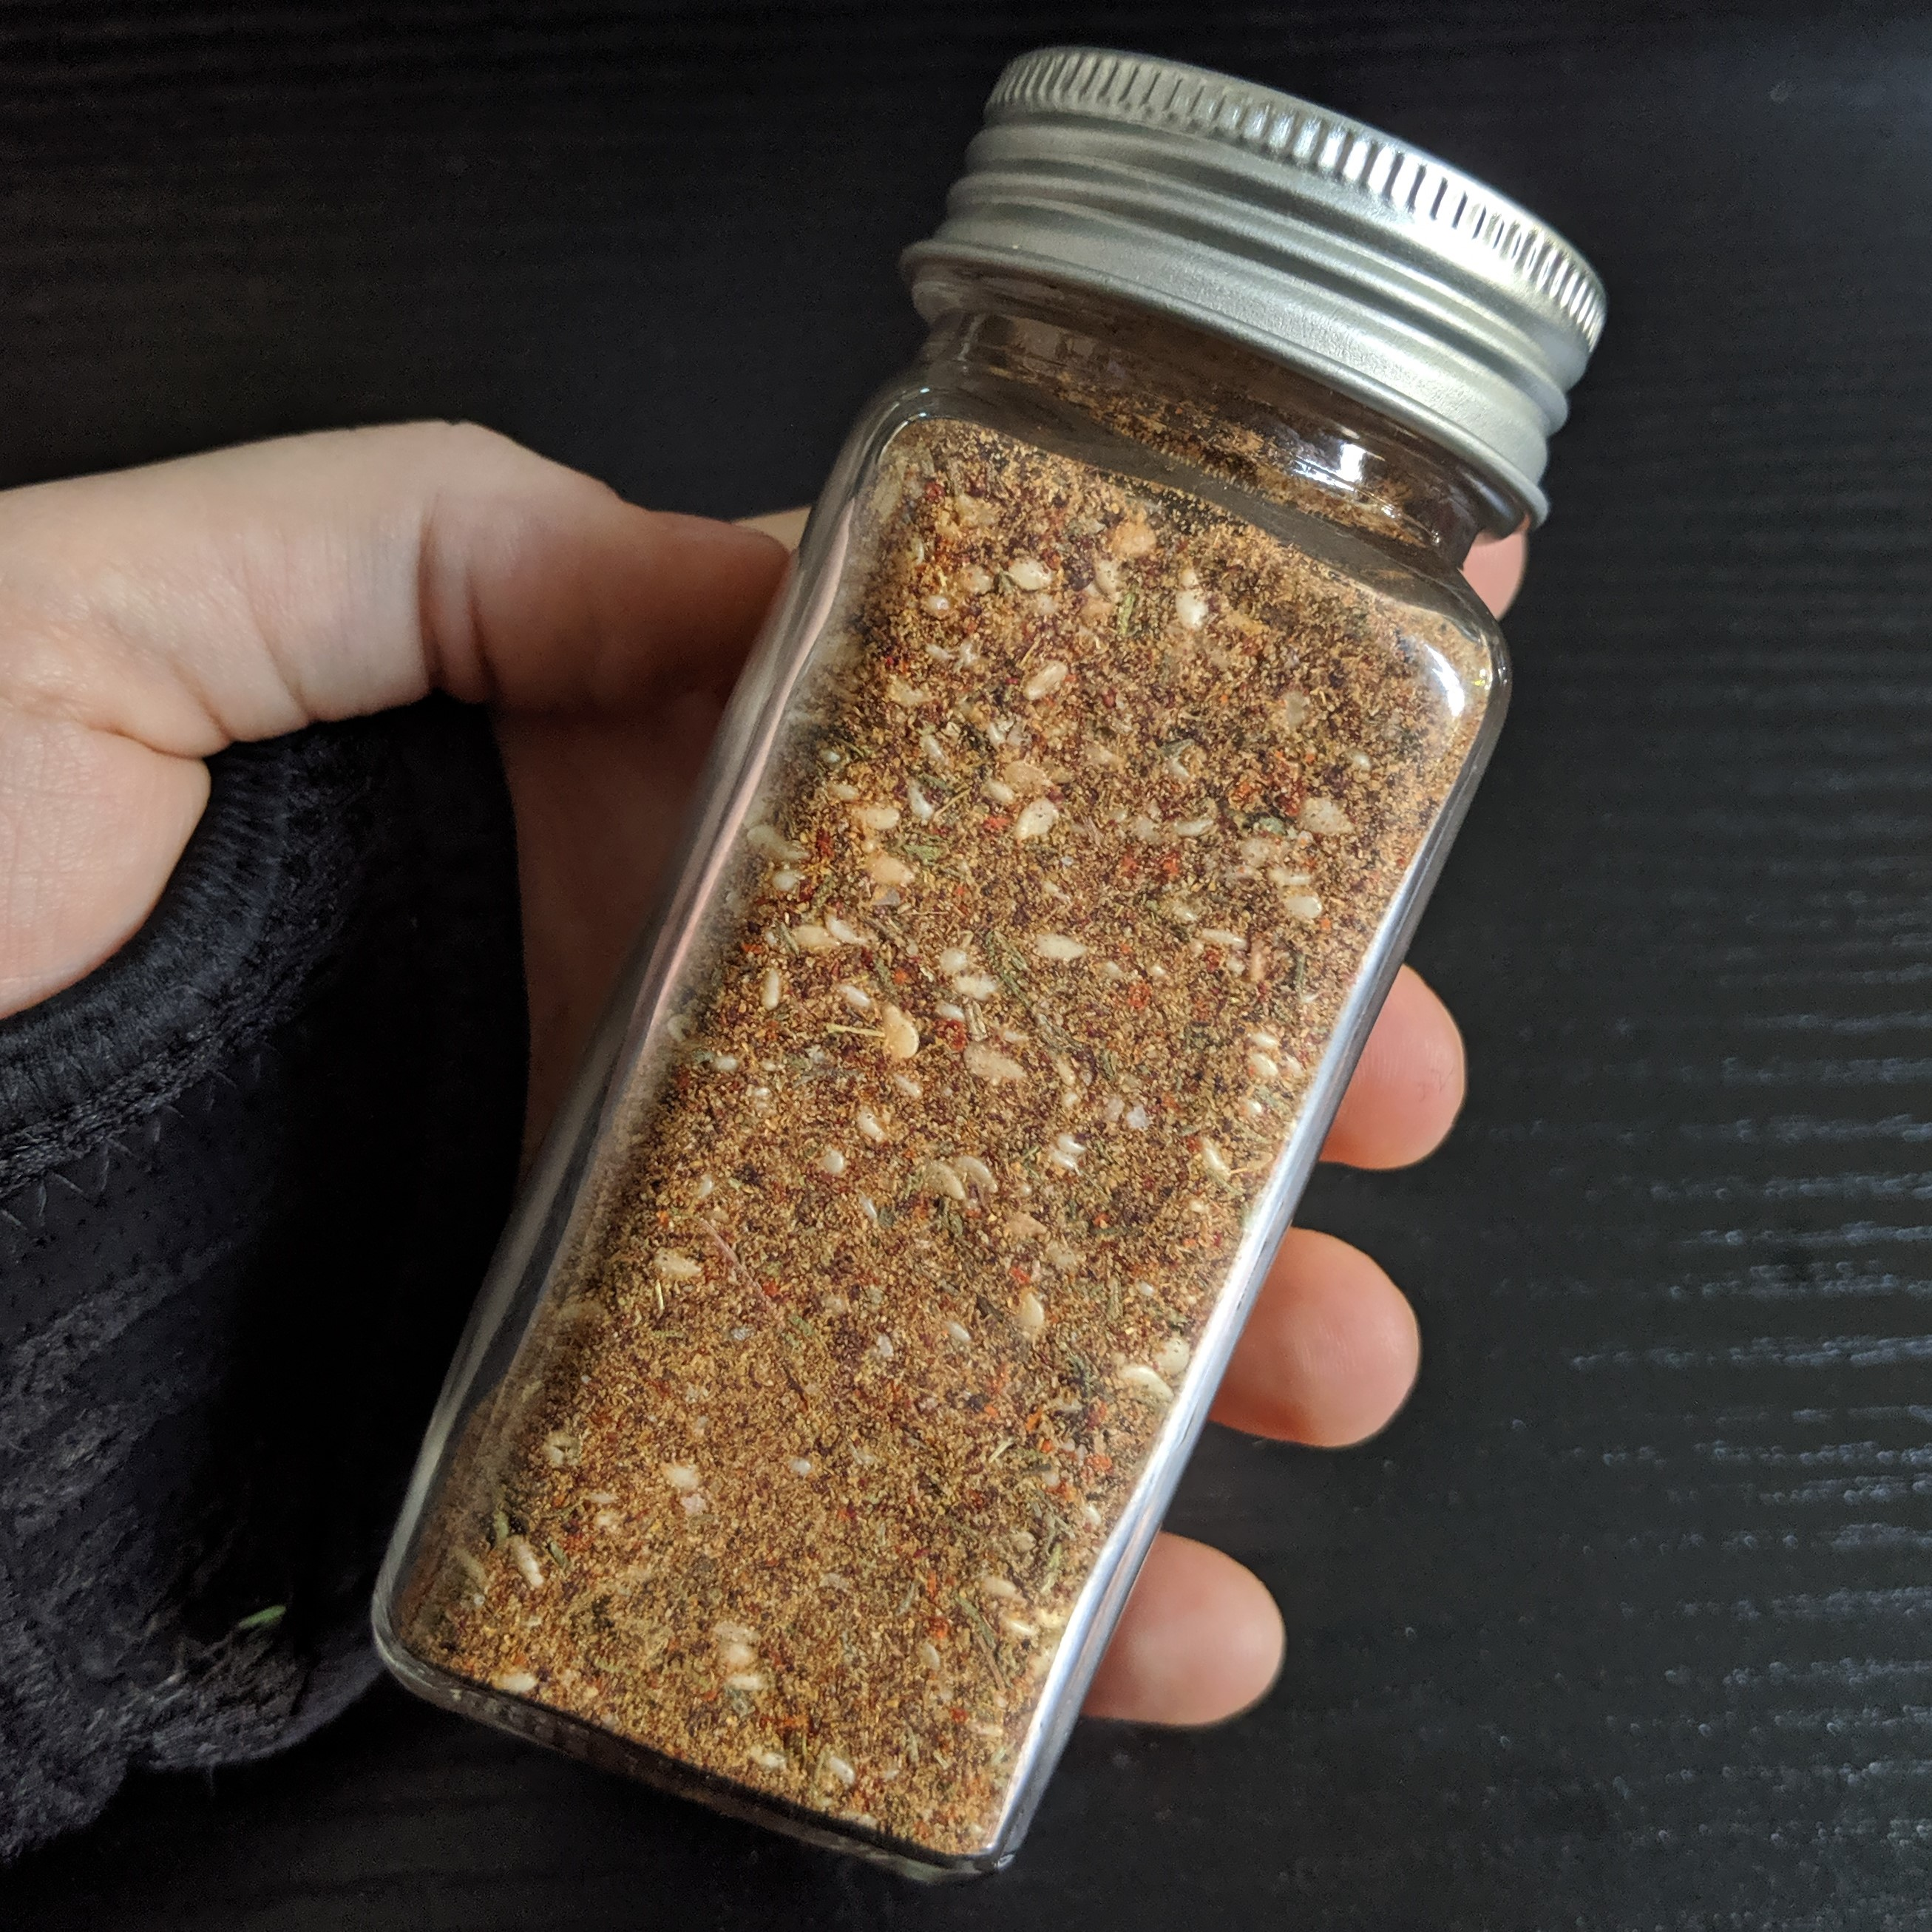
\includegraphics[width=0.15\textwidth]{zaatar-spice}}}\end{floatingfigure}\begin{huge}Za'atar Spice\end{huge}\newline\vspace{-2.5mm}\newline\renewcommand{\arraystretch}{1.1}\begin{tabular*}{\textwidth}{@{\extracolsep{\fill}}lr}A Middle Eastern spice mixture with some heat\\Sunny C\end{tabular*}\newline\vspace{10mm}\newline\begin{huge}Ingredients\end{huge}\\\rule[2.8mm]{\textwidth}{.1pt}\vspace{-3mm}\begin{itemize}\item 2 tbs toasted ground cumin\item 2 tbs toasted ground coriander\item 2 tbs ground sumac\item 2 tbs dried thyme\item 2 tbs toasted sesame seeds\item 1 teas kosher salt\item $\frac{3}{4}$ teas aleppo chili flakes\end{itemize}\vspace{7mm}\begin{huge}Directions\end{huge}\\\rule[2.8mm]{\textwidth}{.1pt}\vspace{-3mm}\begin{enumerate}\item Mix spices together in a small bowl. Store in an airtight container.\end{enumerate}\end{document}